% ---------------------------------------------------------------------
%  Sample content: code, tables, figures and algorithms
% ---------------------------------------------------------------------
\section{Code}\label{sec:code}

A whole source file, with line numbers and the file name as the title:

\pyfile{code/example.py}

Program output in a terminal block:

\begin{terminal}
$ python code/example.py
mean = 5.00, std = 2.00
\end{terminal}

Any language supported by the \code{listings} package:

\begin{codeblock}{C++}[main.cpp]
#include <iostream>

int main() {
    std::cout << "Hello, world!" << std::endl;
    return 0;
}
\end{codeblock}

% ---------------------------------------------------------------------
\section{Tables and figures}\label{sec:tables}

Tables and figures stay exactly where they are written. The first row of a
table is the header; the rows below it are striped automatically.

\begin{datatable}[A striped table][tab:sample]{lccr}
\thead{Item} & \thead{Group} & \thead{Status} & \thead{Value} \\
\midrule
Alpha & A & done & 12.5 \\
Beta  & A & open &  8.0 \\
Gamma & B & done & 15.2 \\
Delta & B & open &  4.7
\end{datatable}

\begin{widetable}[A full-width table with wrapping text][tab:wide]{lLl}
\thead{Element} & \thead{Description} & \thead{Example} \\
\midrule
Box     & Numbered content with an optional title and a label for references. & \code{theorem} \\
Callout & Unnumbered side note with an icon, in one of six colors.            & \code{warning} \\
Code    & Highlighted source code with line numbers and a file name.          & \code{python}
\end{widetable}

\begin{notefigure}[A plot drawn with pgfplots][fig:plot]
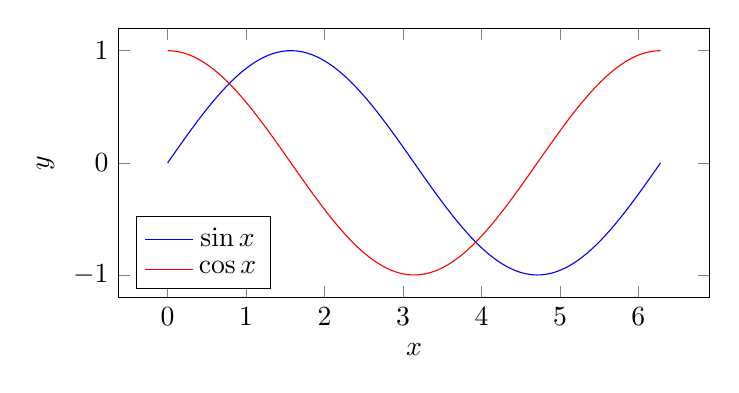
\begin{tikzpicture}
\begin{axis}[width=0.75\linewidth, height=5cm, xlabel={$x$}, ylabel={$y$},
             domain=0:6.283, samples=100, legend pos=south west]
  \addplot+[no marks] {sin(deg(x))};
  \addplot+[no marks] {cos(deg(x))};
  \legend{$\sin x$, $\cos x$}
\end{axis}
\end{tikzpicture}
\end{notefigure}

\begin{notefigure}[Images from files, side by side][fig:images]
  \begin{subfigure}{0.32\linewidth}\centering
    \includegraphics[width=\linewidth]{example-image-a}\caption{First image}
  \end{subfigure}\quad
  \begin{subfigure}{0.32\linewidth}\centering
    \includegraphics[width=\linewidth]{example-image-b}\caption{Second image}
  \end{subfigure}
\end{notefigure}

% ---------------------------------------------------------------------
\section{Algorithms}\label{sec:algorithms}

\begin{algorithm}[H]
\caption{A generic iterative procedure}\label{alg:sample}
\begin{algorithmic}[1]
\Require input data $D$, tolerance $\varepsilon > 0$
\Ensure result $r$
\State $r \gets$ initial guess
\Repeat
  \For{each item $d \in D$}
    \State update $r$ using $d$
  \EndFor
\Until{the change in $r$ is smaller than $\varepsilon$}
\State \Return $r$
\end{algorithmic}
\end{algorithm}

% ---------------------------------------------------------------------
\section{Cross-references}\label{sec:refs}

Every labeled element can be referenced by name and number, and each
reference is a link: \cref{def:sample}, \cref{thm:sample}, \cref{ex:sample},
\cref{eq:sample}, \cref{tab:sample}, \cref{fig:plot}, \cref{alg:sample} and
\cref{sec:math}.

\begin{summary}
One style for notes, books and slides. Replace the sample content with your
own and keep the structure.
\end{summary}
